\documentclass{article}
\usepackage{amsmath}
\usepackage[fleqn]{mathtools}
\usepackage{amssymb}
\usepackage{amsthm}
\usepackage{enumitem}
\usepackage{float}
\usepackage[dvips,xetex]{graphicx}
\usepackage{caption}
\usepackage{subcaption}
\usepackage[linesnumbered,ruled]{algorithm2e}
\usepackage{xcolor}
\usepackage{setspace}
\usepackage[margin=1.25in]{geometry}

\begin{document}
	\title{Multi-actor network repair problems in a post-hurricane context}
	\author{Brian French}
	\maketitle
	\section{Status Tracker}
	\begin{itemize}
		\item Introduction -- drafted+1 set of revisions
		\item Literature Review - drafted+1 set of revisions
		\item Modeling - drafted+1 set of revisions
		\item Results/conclusions -drafted but ongoing expansion/revision
		\item Resilience -- Drafted
		\item Conclusions -- drafted
	\end{itemize}
	\doublespacing
	\section{Introduction and Motivation}
	Hurricanes are a growing concern in the operation of power grids in coastal areas. This is due partly to the increasing density of cities in coastal areas, but the impacts of climate change are causing both rising sea levels making flooding worse. Combined with the effects of climate change directly, there is also the indirect effect of water warming causing more frequent and more severe hurricanes \cite{MannEA2006}. This phenomenon suggests that repair procedures and resilience planning for hurricanes will be of increased importance in the coming years.
	
	This thesis explores the gap in existing literature where previous efforts have not explicitly considered how multiple networks depended on each other for the logistics of repair, particularly the post-disaster infrastructure recovery interactions between power grid and road networks. For example, to repair a damaged power grid element, the element must be accessible to the crew attempting to repair it. Moreover, the crew will take time to go from one element to the next to repair, affecting the rate of restoration power grid's performance during recovery as time is lost in transit. This implies that the road network (how damaged it is and how its recovery is planned) becomes part of the overall recovery efforts for logistics, supply delivery, as well as power grid repair. During a hurricane, the road network will sustain substantial damage from flooding and/or debris on the road surface, which necessitates road grid repairs/clearance as well. To handle the issues of repairing power grids in a way that minimizes the amount of disruption to power service, both types of repairs (road network and power grid) should be considered jointly. To capture the joint interaction of these two networks, we consider the route that repair crews take on the road network as they effect repairs to either the roads or the power grid. Previous literature does not study this specific interaction as discussed in the section below.

	Understanding of repair efforts on power grids begins with understanding the basics of power grid topology. We divide the power grid into transmission and distribution networks. Transmission consists of generators, buses/substations, and high voltage connecting lines. Because this side of the grid has multiple sources and sinks, power is not guaranteed to flow in a certain direction. The distribution side of a network begins at the bus/substation level and connects end users of power to the grid as a whole. Because power flows from the substation to the end user in a single source network, these networks are comparatively simpler to model. For the sake of this thesis, we restrict ourselves to the transmission level power grids as distribution grids are simpler at an electrical level as well as being geographically small enough that ignoring routing time costs does not stray from optimality very far. In addition, as distribution level damage happens in routine storms, power utilities have a better understanding of how to handle this damage due to experience. In addition to the practical concerns of how these power grid levels differ, the scale of service loss is dramatically different. Loss of distribution power lines can lead to loss of power service to small segments of a neighborhood while loss of a substation or set of transmission lines can knock out power to several neighborhoods or entire towns depending on the extent of redundancies.
	
	
	\section{Literature Review}
	\subsection{Hurricane Damage Modeling}
		When delving into the background literature, no discussion of modeling repair after a hurricane can happen before looking at the literature on damage to power grids from hurricanes. A paper by Guikema et al\cite{GuikemaEA2010} uses a model based on negative binomial regression to estimate the number of downed power lines in combination with a classification tree handling flooding and wind speed over/under 100 miles per hour as a second method for estimation for damage severity. A paper by Scherb et al \cite{ScherbEA2015} on the other hand takes an approach more rooted in scenario generation and tries to use the peak wind speed and proximity to the eye wall of a hurricane to construct a loss function (a function that maps wind speed onto probability of damage for a given element) for power lines. Both of these papers come to the similar conclusion that damage to 40-70\% of the power lines in the network due to wind and thrown debris is common in hurricanes. Damage is geographically distributed based on proximity to the eye-wall of a hurricane, but because hurricanes are frequently hundreds of miles across, damage inside of a single city may appear functionally random due the small geographic area experiencing basically the same peak wind speed. 
		
			\begin{figure}[htbp]
			\centering
			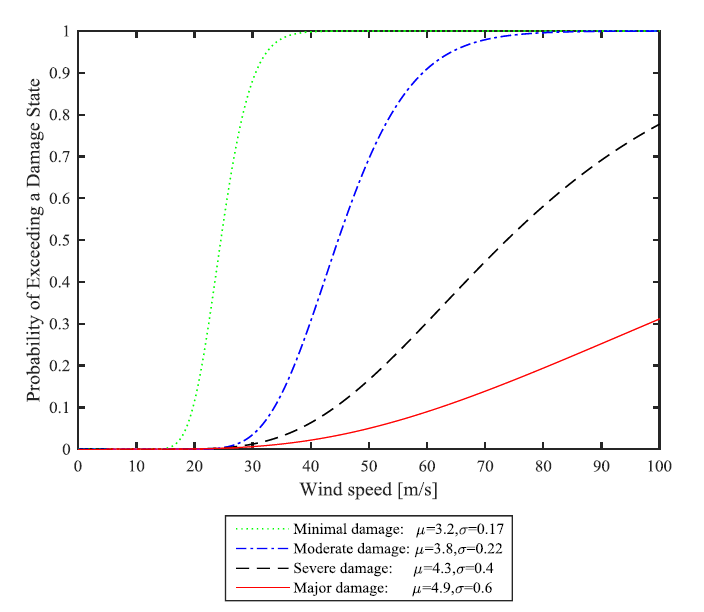
\includegraphics[width=.5\linewidth]{ScherbFigure.PNG}
			\caption{A power line loss function example from the paper by Scherb et al}
		\end{figure}
		
		 Winkler et al \cite{WinklerEA2010} Provide the most thorough analysis of these 3 papers using real world topographies from various small regions of Texas and coming up with loss functions for both lines and substations. Worth noting in all three of these examples is that lines and substations sustain the most damage, but generators themselves are robust enough that a hurricane is unlikely to damage them. This means they can be ignored in the repair modeling later on. This validated the later modeling of how damage happens to a power grid in the wake of a hurricane that neglects to consider the impact on power generation.
	\subsection{Existing Power Grid Repair Modeling}
		Power grid repairs in the wake of hurricanes are reasonably well studied area of research. Ang \cite{NPSMasters} solves a scheduling problem of power grid repair in the wake of both hurricanes and terrorist attacks. The problem is just in which order should elements be repaired with little consideration of the actual logistics of getting crews to the sites where power grid repair can happen. While they don't consider impacts of roads, they do significant work in extending repair models to DC power flow based models of the power grid when covering how to model a damaged power grid. Along similar lines, Arab et al \cite{ArabEA2015} solve a similar problem under uncertainty by treating the state of each power line and generator as a random Bernoulli variable and solving the ensuing stochastic optimization problem. Though it solves the problem as a two stage stochastic program with recourse and treatment of the hurricane damage is much better, there is still no consideration of repair logistics. 
		
		A paper by Ouyang et al\cite{OuyangEA2014} does a statistical analysis of the rate at which damage is recovered in the context of broader power grid resilience. While more descriptive than prescriptive, they do lay out that transmission grid repairs take priority alongside "critical facilities vital to public safety, health, and welfare". Of note in this paper is that they identify that much of the existing literature on repairs to power grid is based on descriptive studies of statistical repair times rather than model-driven optimization models for how to improve that process.
		
		Golari et al\cite{GolariEA2014} take a different approach to ensuring power demand satisfaction in the context of a damaged power network by approaching the problem in the lens of construction of sub-grids (termed "islands" in much of the electrical engineering literature) in order to keep demand satisfied in a post-disaster context. This is done by solving a two stage stochastic program in order to identify the best sub-grids to construct under the uncertainty of a set of contingencies. Islanding is an active field of study in power grid engineering for generating tools to minimize the impact of disaster damage. A paper by Panteli et al\cite{Panteli2016} studies disaster damage by constructing islanding plans in a way that would minimize load loss subject to severe weather. Though there is no consideration of repair, their modeling warrants the importance of resilience as an area of study.  A follow on paper to that by Nobels and Panteli \cite{NobelsEA2019} extends the previous work of the resilience of islanding on IEEE 30 and 57 bus test networks to cascaded failures caused by disasters as well as differentiating intentional vs unintentional load shedding due to the disaster.
	\subsection{Existing Road Grid Repair Modeling}
		A paper by Pregnolato et al\cite{PregnolatoEA2017} provides an overview of probability of road damage by location and intensity. They go on to provide a literature review and meta-analysis of existing papers in the subfield. They then go on to summarize a variety of versions of depth-disruption functions for roads based on local rain intensity. Alone this paper doesn't add significant amounts to modeling repair efforts as the models provided for road repair are cursory, but the analysis of damage to road networks from debris and flooding in the wake of a disaster is covered in depth.
		
		Looking next at how previous papers have addressed modeling flooding and how to interact with it in a repair context, we start with \cite{DuqueEA2016}. This paper focuses on distribution of relief supplies, but in the context of the problem of supply distribution they consider repair of flooded or damaged roads. Though they solve the problem with dynamic programming rather than the mixed integer programming of similar papers the idea of repair of roads by traversing them at additional cost is the main contribution of their modeling approach.
		
		Also of note from the perspective of road repair is a paper by Aksu et al \cite{AksuEA2014}. Again it is not a paper focused focused on direct repair of networks, but rather a paper focused on evacuation and accessibility to areas flooded by the a disaster. This provides additional insight into flooding and relief as well as a different treatment of the problem using mixed integer programming rather than the dynamic programming of Duque et al. Both of these treatments though cover short term road clearance in the context of disaster. 
		
		All three of these papers make similar assumptions in that minor damage to road networks can be repaired in a time horizon relevant to immediate post-disaster response. While more severe damage to roads can require resurfacing or replacement of bridges, debris and flooding clearance is distinct from those repairs.
	
	\subsection{Resilience}
		As this thesis deals partly with resilience, we look to the corresponding literature for how to define resilience in the context of disaster response for power grids. Molyneaux et al provide\cite{MolyneauxEA2016} a multi-disciplinary literature review of power grid resilience. They broadly define resilience as "capacity to cope with the unexpected". While they go through multiple measures for resilience they use primarily metrics of price. For example, they reduce power flow to the cost of power and the change in cost rather than treating the utility of lost power load directly. Panteli et al \cite{Panteli2017} focus on more specific resilience definitions in the context of disaster response. They focus on both magnitude of drop in service as well as time dependent total loss of power demand satisfied.
		
		Much of the literature on resilience for power grids comes from study of protection from directed attack. Relevant among these is a paper by Deka et al \cite{Deka2018} which provides a study of not just initial damage but potential damage stemming from cascading damage as well identification of elements crucial to construction of resilient power networks. More relevant to this thesis is \cite{Salmeron2004} for their work identifying key resilience elements in the context of mixed integer programming using a DC-powerflow based model of power grids. They solve a bilayer optimization that involves minimization of the maximum satisfied power to determine optimal interdiction.


	
	\section{Repair Problem}
	
	\subsection{Overview}
	To motivate the problem, we see from the literature a gap in looking at power grid repairs in a post-disaster context with consideration of the roads. The Federal Emergency Management Agency's 2017 post season after action report\cite{FEMA2017AAR}  and Hurricane Sandy after action report \cite{FEMASandyAAR} make note of the need of increased coordination between agencies for the sake of logistics as well as it having been a major short coming in the repair effort.
	
	We know from the earlier referenced literature that road repair is a concern in the wake of a hurricane. We assume for the sake of this thesis that all roads can be cleared. Clearing here represents digging out drainage for minor flooding and clearing debris. Severely damaged roads should be treated as completely impassible and dropped from the graph representation of the network to allow this assumption to work in a practical context. While repair of these more severely damaged roads can happen, it frequently represents involved construction efforts spanning weeks or months after a disaster and therefore is beyond the scope of the current modeling efforts.
	
	We assume also that the resulting road network for the area corresponding to the power network's service area can be represented with a Watts-Strogatz network, which is a network that connects each node of a graph to the $k$ nearest neighbors and then has probability $p$ of connecting any two nodes chosen. These networks exhibit "small world" property where any two arbitrarily distant nodes can be connected using only a small number of edges. Based on the literature on statistical analyses of road network topologies \cite{LammerEA2006} \cite{ChanEA2011} this is a serviceable but imperfect assumption. Ideally the real topology of a hurricane struck area should be used, but for a computational and modeling effort to draw insight into joint repair efforts, the contrived Watts-Strogatz based network suffices. We then apply damage to this network to allow for the solution of interacted road and power repair problems to better study the impact of considering these two aspects together.
		
	We model time in discrete shifts here because it allows for mixed-integer programming to be used as a tool to solve both problems. It additionally allows for easier interaction of both sides (Road and Power) of the problem by operating them on the same time chunks. 
	
	We also assume that direct current (DC) approximations of power flow can be used to approximate the full alternating current (AC) power flow of a real power grid. We know that representation of DC power flow is more accurate than just a "pipe-flow" representation of a power grid as it captures some of the physics behind electrical flows. This interaction may be important in the consideration of repair and resilience as DC power flow models spread flow out among possible lines whereas pipe-flow style models load all of the demand onto single lines as a byproduct of they're solved. DC representation is usually within 5-10\% of the AC power flow solutions \cite{Frank2016} \cite{StottEA2009} meaning that it suffices for the sake of the power repair problem. As the problem we're considering is one of logistics and not one of power flow management, an approximation in the power flow relaxes numerical accuracy of the power flow but leaves a near optimal schedule that still minimizes load shed over the repair horizon. Because demand at each node/bus is based on pre-hurricane power demand, a somewhat coarse approximation is accurate enough.  
	
	With the power grid, we elect to ignore distribution below the substation level. Each substation has a distribution level network that services the local area (e.g plugging the grid into a house), but the wires between substations are considered the transmission level network. Discarding the distribution network in the modeling of repair scheduling stems from two factors. First that it's geographically very co-located damage so that including road networks would provide little benefit, and secondly, flow at the distribution level goes from the substation as a source to the demand sites as a sink. This necessitates different modeling than the transmission grid because potential changes in direction as power flow from A to B and from B to A can be valid at different times on the transmission grid.
	\subsubsection{Validating use of DC power flow}
	
	From a review of the literature of earlier power network related operations research problems, many of them relax one step further than DC powerflow all the way to traditional network flow or "pipe-flow" models that resembles any abstracted network. For these problems, DC powerflow models are likely considered to be overkill upon first glance and therefore begs the question of why use it over a traditional network flow model. We define traditional network flow to consist of just flow balance and line limits (analogous to relaxation of constraint (2) in the DCOPF model below). To begin with, DC power flow tends to spread power flow out more across lines due to the physics of the grid while a network flow model tends to seek an extreme point solution which leads to fewer lines under use, but heavier loading on those lines. To demonstrate this, we solve DCOPF and it's corresponding relaxation of constraint (2). The results shown below aren't quite as drastic as initially expected, but there is a noticeable difference between flow patterns, and when looking at multiple cases of damage to the power grid, it may become relevant, and as a result is worth including into models. In addition to this, the computational cost of including DC power flow over a pipe-flow model is near zero and helps keep math representation of the network closer to the real AC flow. This has the added benefit of making it easier to persuade practitioners in the field that the models presented using DC power flow have relevance.
	
	\begin{figure}
		\centering
		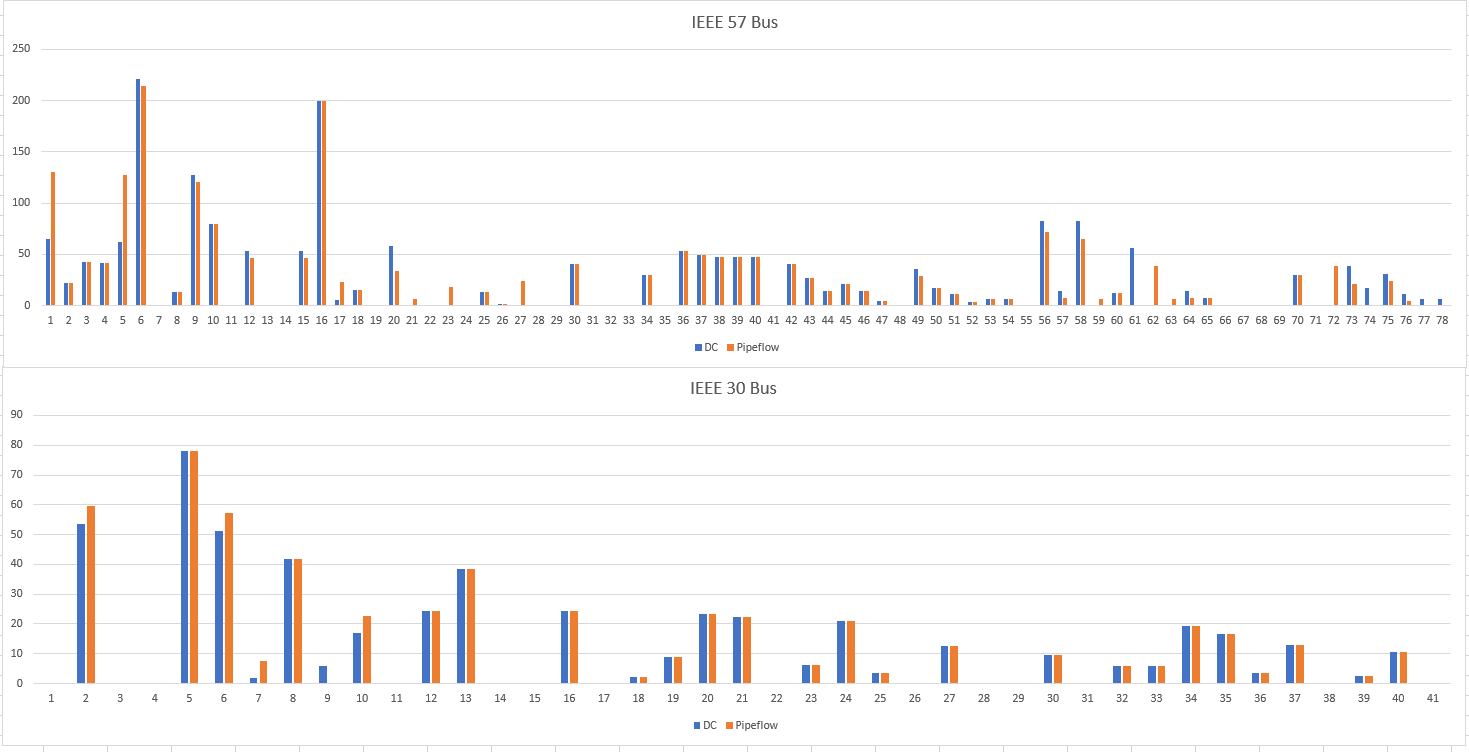
\includegraphics[width=\linewidth]{DCvsPipeflow.PNG}
		\caption{Comparison of DC and traditional (pipeflow) network flow}
	\end{figure}
	
	Further, as we extend this model into resilience, use of pipeflow style network models to handle power flow may over-prioritize the resilience of certain lines as a false conclusion. Since DC powerflow is of low computational cost and low model complexity to add and has upside in some limited cases, we find its inclusion to be warranted.
	\subsubsection{DCOPF}
		To begin looking at methods of studying repair of damaged power grids, we first must understand the Direct Current-Optimal Power Flow (DC-OPF) model as it forms the basis of all more complex power models used in this thesis. The power grid can be represented as a mathematical graph with edges representing power lines and the nodes of the graph corresponding to substations that service a distribution area
		
		
		We use the following notation for clarity in models
	\begin{itemize}
		\item $o(e)$ is the node at the origin of line e
		\item $d(e)$ is the node at the destination of line e
		\item $O(i)$ is the set of lines with origin i
		\item $D(i)$ is the set of lines with destination i
	\end{itemize}
	We define the following parameters and sets
	\begin{itemize}
		\item $i \in N$ is the set and indexer for nodes
		\item $e \in E$ is the set and indexer for edges
		\item $C_i$ is the cost of producing one unit of power at node i
		\item $P_i$ is the maximum power generation for node i. If there is no generator, maximum production is zero watts.
		\item $D_i$ is the demand for power at node i
		\item $B_e$ is the line susceptance for power line e (susceptance is the measure of ease of power flowing along a line)
		\item $\underline{L_e}$ is the maximum amount of flow on line e
	
	\end{itemize}
	We also have the following decision variables
	\begin{itemize}
	\item $X_e$ is the power flow on line e (flow is based on lower indexed node to higher indexed node, so negative flow is allowed and represents flow from the higher indexed node to the lower indexed node)
	\item $G_i$ is the power generated at node i
	\item $\theta_i$ is the phase angle for power flow at node i 
	\end{itemize}
	The model can then be formulated as 
	\begin{equation}
\textnormal{Minimize} \sum_{i\in N} C_i G_i
	\end{equation} 
	subject to
	\begin{eqnarray}
	X_e = B_e (\theta_{o(e)} - \theta_{d(e)}), \hspace{4pt} \forall e \in E\\
	G_i - \sum_{e \in O(i)} X_e + \sum_{e \in D(i)} X_e = D_i, \hspace{4pt} \hspace{4pt} \forall i \in N\\
	  G_i \leq P_{i} \hspace{4pt} \hspace{4pt} \forall i \in N	\\ 
	  -\underline{L_e} \leq X_e \leq \underline{L_e}
\end{eqnarray}

To explain, the problem is how to generate power at the minimum cost in a way that satisfies all of the demand subject to the physics of how power grids operate. As a byproduct, this problem also solves out line flow amounts and phase angles for each node as expressed in a per unit basis. Constraint $2)$ is part of the DC approximation to AC power flow where we assume $sin(x) = x$ for small values of x and reduce power flow to just its real component (dropping the reactive component of power flow) and the aforementioned linear approximation of phase angle. The representation of power flow tracks only power demand (wattage) and neglects voltage as voltage control of power grid is a well solved problem in electrical engineering literature. Constraint $3)$ is a standard flow balance constraint (i.e power going into a node has to be equal to power coming out of node). Constraint $4)$ restricts generation to the maximum for the generator. Constraint $5)$ is a flow capacity constraint on each power line. While overall a simple problem, DCOPF serves as the building block for most of the power grid models used for the rest of this thesis as well as being used in practice for controlling power grid generation and dispatch. \cite{LiBo2007}. 
	
	
	\subsection{Road Repair Problem}
	When dealing with repairs on the power grid, we need a framework for solving problems based on the damage to the road network. We elect to solve this a problem as a scheduling/routing problem for a crew tasked with clearing debris and/or digging out minor flooding, we take inspiration from Duque et al \cite{DuqueEA2016} and their treatment of how road repairs function in practice using routing the crew down a damaged road at higher time cost . This takes the form of constructing a series of roads to traverse as tour that begins and ends at a depot.
	
	We model this as per the following:
	
	Parameters and Sets:
	\begin{displaymath}
	\begin{array}{ll}
	T & \mbox{the set of time periods (shifts) over the time horizon, indexed by $t$}\\
	N & \mbox{the set of nodes in the graph, representing the intersections of road segments}\\
	c_{ij}^t & \mbox{measure of the value of the road segment from node $i$ to node $j$ during period $t$}\\
	l_{ij} & \mbox{is the transit time of the road segment between nodes $i$ and $j$ under nominal conditions}\\
	r_{ij} & \mbox{time to repair the road segment between nodes $i$ and $j$ (hours), including travel time}\\
	s^t & \mbox{the length of period $t$ in time units (hours)}\\
	o_{ij} & \mbox{initial condition of the road segment between nodes $i$ and $j$}\\
	\end{array}
	\end{displaymath}
	
	and Decision Variables
	
\begin{displaymath}
\begin{array}{ll}
X_{ij}^t & \mbox{binary variable for road segment $ij$ being operational in time $t$}\\
K_{ij}^t & \mbox{binary variable for travel from $i$ to $j$ being in the tour at time $t$}\\
S_{ij}^t & \mbox{length of travel for road segment $ij$ at time $t$}\\
\end{array}
\end{displaymath}	
\begin{equation}
\min \sum_{t \in T}  \sum_{i,j \in N} c_{ij}(1-X_{ij}^t) 
\end{equation}
subject to:
\begin{eqnarray}
\sum_{i,j \in N} S_{ij}^t K_{ij}^t \leq s^t, \hspace{6pt} \forall t\in T \\
S_{ij}^t = \max \{l_{ij}, r_{ij}(1-X_{ij}^t) \}, \hspace{6pt} \forall t\in T, \hspace{5pt} \forall i,j \in N\\
\sum_{j \in N} K_{ij}^t - \sum_{j \in N} K_{ji}^t = 0, \hspace{6pt} \forall t\in T, \hspace{5pt} \forall i \in N\\
X_{ij}^t \le \sum_{t'=0}^{t-1} K_{ij}^{t'} + o_{ij} , \hspace{6pt} \forall t\in T,  \hspace{5pt} \forall i,j \in N\\
\sum_{i,j \in S; i\neq j} X_{ij}^t \leq |S|-1, \hspace{6pt} \forall S \subset N, \hspace{2pt} S \neq \emptyset, \hspace{5pt} \forall t\in T.
\end{eqnarray}

Of note is that constraint 7) is nonlinear as intuitively expressed. We linearize it by rewriting constraints 7) and 8) as the following:

\begin{eqnarray}
\sum_{i,j \in N} S_{ij}^t \leq s^t, \hspace{6pt} \forall t\in T \\
S_{ij}^t \leq M*K_{ij}^t \hspace{6pt} \forall t\in T, \hspace{5pt} \forall i,j \in N\\
S_{ij}^t \geq l_{ij}K_{ij}^t \hspace{6pt} \forall t\in T, \hspace{5pt} \forall i,j \in N\\
S_{ij}^t \geq (1-X_{ij}^t)r_{ij} - (1-K_{ij}^t)M \hspace{6pt} \forall t\in T, \hspace{5pt} \forall i,j \in N
\end{eqnarray}

To explain the modeling, the objective is to minimize the value of out-of-service road. Without loss of generality, this can be substituted with a set of priority weights from another agency that cares about the road network's operation. For example, the value of given road segments to an agency like the Red Cross or FEMA that is tasked with bringing relief supplies in to a disaster-stricken area

Constraint 7) provides a scheduling constraint limiting the tour's length to the length of the shift. Constraint 8) is a nonlinear but linearizable constraint that sets the length of a road to either its nominal operation time or its repair time depending on whether or not it is marked as working (e.g $X_{ij}^t$ = 1). Constraint 9) is a standard path connectivity constraint. Constraint 10) restricts each road segment to only be working if it started working or has been repaired, and Constraint 11) is a standard set of subtour elimination constraints.
	\subsection{Power Grid Repair Problem}
	When looking at repair of the power grid, we formulate a discrete time mixed integer program that captures both the planning/scheduling/movement of repair crews as well as the DC power flow model. We assume the following:
	\begin{itemize}
		\item Repair of a power line can be started from either end of that power line.
		\item Minimum spanning tree's lower bound provides a usable approximation for the sake of keeping model runtime down 
		\item Load shedding can be modeled as a continuous loss even though on real power grids it's a series of discrete decisions that allows small increments of load shed, though not truly continuous power shedding.
	\end{itemize}
	We pose the model as follows:

	\begin{displaymath}
	\begin{array}{llll}
	N & \mbox{set of nodes, indexed by $i$} \\
	E & \mbox{set of power lines, indexed by $e$}\\
	R & \mbox{the set of road segments} \\
	T & \mbox{the planning horizon, indexed by $t$}  \\
	O(i) & \mbox{set of lines with origin $i$} \\
	D(i) & \mbox{set of lines with destination $i$} \\
	o(e) & \mbox{origin node of line $e$} \\
	d(e) & \mbox{destination node of line $e$} \\
	\underline{L_e},\overline{L_e} & \mbox{power lower and upper bounds for line $e$}\\
	\Delta_{i} & \mbox{time to repair node $i$} \\
	\delta_{e} & \mbox{time to repair line $e$}\\
	C_{SP(i)} & \mbox{length of the shortest path from depot to node $i$}\\
	D_i & \mbox{power demand at node $i$ in the pre-disaster state}\\
	P_k & \mbox{maximum power generation for generator $k$}\\
	B_e&  \mbox{line susceptance for power line $e$}\\
	I_e, I_i & \mbox{initial condition of line $e$ and node $i$, respectively}\\
	X_{e}^{t} & \mbox{power flow on line $e$ at time $t$}\\
	G_{k}^t & \mbox{production from generator $k$ at time $t$}\\
	Y_{n}^t & \mbox{Load shed from bus $n$ at time $t$}\\ 
	V_i^t & \mbox{indicator for node $i$ functioning at time $t$}\\
	W_{e}^t & \mbox{indicator for line $e$ functioning at time $t$}\\
	S_{e}^t & \mbox{indicator for line $e$ serviced at time $t$}\\
	F_i^t & \mbox{indicator for node $i$ serviced at time $t$}\\
	\theta_i^t & \mbox{phase angle for the power flow at $i$ in time $t$}\\
	MST_t & \mbox{length of the tree used for ``routing'' at $t$} \\
	Z_{ij}^t & \mbox{indicator for $ij$ being in the spanning tree at $t$}
	
	\end{array}
	\normalsize
	\end{displaymath}
	\begin{equation}
	\min \sum_{i \in N} \sum_{t \in T} (1-V_i^t)D_i
	\end{equation}
	subject to:
	\begin{eqnarray}
	X_e^t = B_e (\theta_{o(e)}^t - \theta_{d(e)}^t), \hspace{5pt} \forall t \in T, \hspace{4pt} \forall e \in E\\
	G_i^t - \sum_{e \in O(i)} X_e^t + \sum_{e \in D(i)} X_e^t = D_i-Y_i^t, \hspace{4pt} \forall t \in T, \hspace{4pt} \forall i \in N\\
	G_k^t \leq P_{k} V_{k}^t, \hspace{4pt} \forall t \in T, \hspace{4pt} \forall k \in N\\
	0\leq S_i^t \leq D_i \hspace{4pt} \forall t \in T, \hspace{4pt} \forall i \in N\\
	D_i (1-V_i^t) \leq S_i^t \hspace{4pt} \forall t \in T, \hspace{4pt} \forall i \in N\\
	\underline{L_e}W_{e}^t \leq X_{e}^t \leq \overline{L_e}W_{e}^t, \hspace{4pt} \forall t \in T, \hspace{4pt} \forall e \in E\\
	\underline{L_e}V_{o(e)}^t \leq X_{e}^t \leq \overline{L_e}V_{o(e)}^t, \hspace{4pt} \forall t \in T, \hspace{4pt} \forall e \in E\\
	\underline{L_e}V_{d(e)}^t \leq X_{e}^t \leq \overline{L_e}V_{d(e)}^t, \hspace{4pt} \forall t \in T, \hspace{4pt} \forall e \in E\\
	MST^t = \sum_{i \in N} \sum_{j \in N} SP_{ij}^t Z_{ij}^{t},  \hspace{4pt} \forall t \in T\\
	\sum_{i \in N} \sum_{j \in N} Z_{ij}^{t} = \sum_{i \in N} F_i^t + \sum_{e \in E} S_e^t - \sum_{i \in N} F_i^t \sum_{e \in O(i)} S_e^t - \sum_{i \in N} F_i^t \sum_{e \in D(i)} S_e^t, \hspace{6pt} \forall t \in T\\
	\sum_{i,j \in S} Z_{ij}^t \leq |S|-1, \hspace{6pt} S \subset N, \hspace{2pt} S \neq \emptyset, \hspace{5pt} \forall t\in T \\
	\sum_{j \in N} Z_{ij}^t \leq F_i^t + \sum_{e \in O(i) \cup D(i)} S_{e}^t, \hspace{6pt} \forall t \in T, \hspace{4pt} \forall i \in N \\
	\sum_{e \in E} \delta_{e}S_e^t + \sum_{i \in N}\Delta_{i}F_i^t + MST_t \le s^t, \hspace{6pt} \forall t \in T\\
	V_i^t \leq \sum_{t'=0}^{t-1} F_i^{t'}+I_i, \hspace{4pt} \forall i \in N\\
	W_{e}^t \leq \sum_{t'=0}^{t-1} S_{e}^{t'}+I_e, \hspace{4pt} \forall e \in E
	\end{eqnarray}
	
	Constraint 13) is the same constraint from the DCOPF model above to handle line susceptance and phase angle related power flow. Constraint 14) is the flow balance constraint from DCOPF with the alteration that demand can be switched on and off at penalty to the objective. Constraint 15) is a generation capacity constraint where generation of power can only flow into the grid if the bus that the generator connects to is intact. Constraints 16-17) handle load shedding from each bus. Constraints 18-20) are flow limit constraints subject to functioning of the line and buses on both sides of the corresponding line.
	
	Constraint 21) defines the length of a minimum spanning tree based on what elements are put in. Constraint 22) is a quadratic constraint that counts how many elements need to be inserted into the minimum spanning tree. Unlike other quadratic constraints, this one is not linearized, but as the quadratic term is due to multiplying two binary decision variables, Gurobi is able to solve these constraints directly. As we're modeling that a line can be repaired from either endpoint, we need to account for the cases where a bus and it's attached node are repaired in the same shift. Constraint 23) is a standard subtree elimination constraint. Constraint 24) restricts the inclusion of elements in the tree to only nodes that have a repair at them. Constraint 25) is a scheduling constraint that matches the one seen in the road repair model, and constraints 26-27) are functionality constraints that restrict operation to things that either started working or have been repaired.
	
	Tying the model in to the operation of power grids, we model loss shedding as a continuous loss to capture the ability of a power utility to disconnect portions of the distribution network in order to reduce the demand on the grid to what can be serviced. In practice, it would be a set of discrete decisions about which parts to disconnect, but relaxing to a single continuous variable captures most of that decision making while not complicating the model to an unreasonable degree.
	
	\subsection{Justifying the use of a Minimum spanning tree approximation}
	The minimum spanning tree usage in the above model we discuss the use of the tree to approximate the route of a repair crew to reduce computational time. We demonstrate this by first formulating the routing version of the problem, then running a pair of scenarios to find first if we get the same (or at least a very similar) answer, and secondly to show the difference in runtime.
	
	We begin by defining our sets and variables as above with the addition of $K_ij^t$ to represent the inclusion of path from $i$ to $j$ in the tour at time $t$. The routing model is then as follows:
	
		\begin{equation}
	\min \sum_{i \in N} \sum_{t \in T} (1-V_i^t)D_i
	\end{equation}
	subject to:
	\begin{eqnarray}
	X_e^t = B_e (\theta_{o(e)}^t - \theta_{d(e)}^t), \hspace{5pt} \forall t \in T, \hspace{4pt} \forall e \in E\\
	G_i^t - \sum_{e \in O(i)} X_e^t + \sum_{e \in D(i)} X_e^t = D_i-S_i^t, \hspace{4pt} \forall t \in T, \hspace{4pt} \forall i \in N\\
	G_k^t \leq P_{k} V_{k}^t, \hspace{4pt} \forall t \in T, \hspace{4pt} \forall k \in N\\
	0\leq S_i^t \leq D_i \hspace{4pt} \forall t \in T, \hspace{4pt} \forall i \in N\\
	D_i (1-V_i^t) \leq S_i^t \hspace{4pt} \forall t \in T, \hspace{4pt} \forall i \in N\\
	\underline{L_e}W_{e}^t \leq X_{e}^t \leq \overline{L_e}W_{e}^t, \hspace{4pt} \forall t \in T, \hspace{4pt} \forall e \in E\\
	\underline{L_e}V_{o(e)}^t \leq X_{e}^t \leq \overline{L_e}V_{o(e)}^t, \hspace{4pt} \forall t \in T, \hspace{4pt} \forall e \in E\\
	\underline{L_e}V_{d(e)}^t \leq X_{e}^t \leq \overline{L_e}V_{d(e)}^t, \hspace{4pt} \forall t \in T, \hspace{4pt} \forall e \in E\\
	Route^t = \sum_{i \in N} \sum_{j \in N} SP_{ij}^t K_{ij}^{t},  \hspace{4pt} \forall t \in T\\
	\sum_{j \in N} K_{ij}^t \geq F_i^t \hspace{4pt} \forall i \in N \hspace{4pt} \forall t \in T\\
	\sum_{j \in N} K_{o(e)j}^t + \sum_{j \in N} K_{d(e)j}^t > S_e^t \forall e \in E \hspace{4pt} \forall t \in T\\
	\sum_{j \in N} K_{ij}^t - \sum_{j \in N} K_{ji}^t = 0 \hspace{4pt} \forall i \in N \hspace{4pt} \forall t \in T\\
	\sum_{i,j \in S} K_{ij}^t \leq |S|-1 \hspace{4pt} \forall S \subset N \hspace{4pt} \forall t \in T\\
	\sum_{j \in N} Z_{ij}^t \leq F_i^t + \sum_{e \in O(i) \cup D(i)} S_{e}^t, \hspace{6pt} \forall t \in T, \hspace{4pt} \forall i \in N \\
	\sum_{e \in E} \delta_{e}S_e^t + \sum_{i \in N}\Delta_{i}F_i^t + Route^t \le s^t, \hspace{6pt} \forall t \in T\\
	V_i^t \leq \sum_{t'=0}^{t-1} F_i^{t'}+I_i, \hspace{4pt} \forall i \in N\\
	W_{e}^t \leq \sum_{t'=0}^{t-1} S_{e}^{t'}+I_e, \hspace{4pt} \forall e \in E
	\end{eqnarray}
	
	We then solve a pair of scenarios that will be discussed more fully later in the thesis to check the validity of the minimum spanning tree assumption. Shown in the table below (Table 1) is objective values and processing times. 
 \begin{table}[htbp]
	\centering
	\begin{tabular}{|c|c|c|}
		\cline{2-3}
		\multicolumn{1}{c|}{} & MST  & Routing \\
		\hline
		Scenario 1 Objective                & $345.2$   & $369.6$   \\
		\hline
		Scenario 1 Runtime                & $25$ seconds   & $639$ seconds \\
		\hline
		Scenario 2 Objectives               & $357.5$   & $406$  \\
		\hline
		Scenario 2 Runtimes              & $15$ seconds   & $488$ seconds \\
		\hline
		Scenario 3 Runtimes (57 bus) & $4328$ seconds & $5400^*$ seconds\\
		\hline
		Scenario 3 Objectives	& $2748$ & No solution due to time limit (22\% gap at 90 minutes)\\
		\hline
	\end{tabular}
	\caption{Runtime and Objective values for MST and Routing versions of the power repair problem}
	\label{time}
\end{table}

From this, we can see that the minimum spanning tree version of the model runs significantly faster and comes to a similar objective. The difference in objective is from one or two elements being scheduled for an earlier shift.

	\subsection{Lower Bounding and Post Processing Heuristic}
	
	From the above models, we also recognize that we can generate a lower bound using these models. By setting all road lengths to zero, we can then generate a schedule for repairs that would satisfy flow constraints and minimize shed demand. This can be post processed into a feasible schedule by starting with the lower bound schedule and then repacking it into shifts using the following algorithm:
	\begin{enumerate}
		\item Begin by assigning shift 1 as the current working shift
		\item Move any repair that hasn't been done that is on the feasible list onto the priority list
		\item Assign any repair from the lower bound's working shift that would occur in the current working shift to the feasible list.
		\item starting from the depot as the current node, calculate the time to reach and repair every element on the priority list from the current node.
		\item if there are unassigned nodes on the priority list that will fit into the current shift, assign the lowest cost node that will. Update the current node to be that node. Go back to step 4 
		\item if there are unassigned edges on the priority list that will fit into the current, assign the lowest cost edge, update the current node, then go back to step 4.
		\item if there are unassigned nodes on the feasible list that will fit into the current, assign the lowest cost node, update the current node, then go back to step 4.
		\item if there are unassigned edges on the feasible list that will fit into the current, assign the lowest cost edge, update the current node, then go back to step 4.
		\item If nothing else will fit into the current shift, increment to the next shift and start from step 2.
		\item Once every repair has been assigned to a shift, end the algorithm.
	\end{enumerate}
	
	This is very similar to most greedy heuristics for knapsack problems just with a linked series of knapsacks. This heuristic runs in polynomial time (for the heuristic itself, the simplified mixed integer program is non-polynomial though fast), and as we show later, it's close to our full solutions in a variety of examples
	
	\subsection{Framework for interacting}
	Now that we've established both models to be used to draw insights from this problem, we now outline how we're going to interact them. Since the models are solved independently, we have to choose one of them to be the first mover and one to be the second mover. We therefore lay out the following frameworks:
	\begin{itemize}
		\item \textbf{Road First}-- To model the problem as if the road grid's actor had priority in the repair effort. This is done by solving the road model, then feeding the solutions into the power model as a time-varying shortest path.
		\item \textbf{Power First} -- To model the problem with the power grid as the first mover, we solve the power grid repair problem with the roads at their nominal length and presume that due to coordination effects the power grid actor the road grid repairs will happen before the road is needed to affect power repairs. To account for this delay while waiting for road repair, we introduce a one shift delay before the start of power repairs.
		\item \textbf{Uncoordinated Repairs} -- To handle the case where the power agency may have to commence repairs with no prior information about the state of the roads. We model the roads as if they are damaged and their state does not change.
		\item \textbf{Heuristic} -- Using the heuristic described above, both road first and power first versions of the problem can be solved to approximation quickly.
	\end{itemize}
	\subsection{Model Runtimes}
	Models are only useful to the point which they are able to be implemented. As disaster response planning is a somewhat sensitive affair, a model that takes days to run isn't useful. Based on using Gurobi 8.1.1 running on a i5-9600k with 32gb of RAM running through the gurobipy interface for Python 3, model runtime for road repairs ranges between 5 and 15 minutes on the 30 node case and 15-45 minutes on the 57 node case depending on damage level (more damage means more possible decision options which means a longer runtime). Power repair ranges between 10-20 minutes for IEEE 30 bus depending on treatment of the road network and 60-90 minutes for IEEE 57 bus.
	\section{Results on Standard test systems}
	\subsection{Introduction to Results}
	To validate the model outlined as more than just a theoretical exercise in modeling, we engineer test cases based on standard IEEE power grids. We choose to use the 30 bus and 57 bus systems \$CITATION GOES HERE in order to capture things on a large enough scale to demonstrate applications for extension into practical uses later on. To convert these from standard test grids to DC versions for use in this model, reactive/imaginary power flow is dropped leaving only real power flow. We then overlay a Watts-Strogatz graph with connection to the 3 nearest neighbor nodes and .03 global connectivity (i.e each node has a 3\% chance of being connected to any other node)as mentioned earlier based on fitting power buses to a grid. The key reason for this is to maintain triangle inequalities where having a network that violates triangle inequalities is both unrealistic to "real world" situation as well as altering the solutions of routing problems \cite{FlemingEA2013}. We plan this so that travel time between opposite sides of the network are about 3 hours so that routing times are not trivial compared to repair times. We arbitrarily define repair times to be 5 hours for damaged nodes representing replacement of easy to fix components like breakers and downed lines inside the substation. More severe damage resulting from flooding and/or corrosion can take months to repair and is therefore outside the scope of immediate post-disaster response. We assume lines have a repair time of 1 hour plus a variable amount based on the geographical distance of the line. We acknowledge these times are somewhat arbitrary, but without loss of generality, data from a power utility can be fed in, so these arbitrary repair times suffice to warrant the utility of the underlying model.
	
	To show validity, we first solve out a base damage scenario for both grid topologies, then conduct perturbations of respectively weather damage, road topology, and damage intensity to show that the model is valid for a large variety of inputs. 
	
	\subsubsection{Base Case}
	Looking at our first case to validate the model, we apply geographically clustered damage to both road and power network. By this, the damage is concentrated where several damaged elements are next to each other in varying locations around the power grid. 
	
	For the base case on the 30 bus network, damage is applied to approximately one third of road segments, one sixth of power buses, and one quarter of power lines. The following repair curves are generated from the model as stated earlier. 
	
	\begin{figure}[H]
		\centering
		
			\centering
			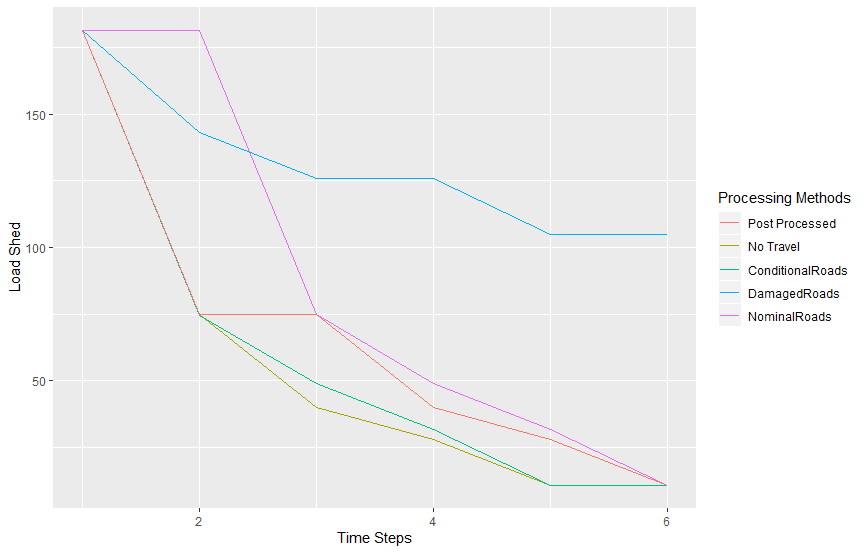
\includegraphics[width=.9\linewidth]{Rplot37.png}9
			\caption{Load Shed by shift in the 30 bus base scenario}
			\label{fig:sub1}
		\end{figure}
	
	We conclude from this that changes in processing and interaction between models has meaningful impact on outcomes. For this case, we find that solving the roads and then conditioning the power repairs on that road schedule yields the outcome closest to the lower bound. This is predicated on the assumption that the road repair crews would need one full shift to get ahead of what roads are needed. If that delay can be reduced, letting the power utility dictate the road repair schedule may become the best schedule.
	
	\subsubsection{Varied Damage location}
	Looking at our next case to validate the mode, we apply randomly distributed damage to both road and power network of similar intensity to the base case.
		\begin{figure}[H]
		\centering
		
		\centering
		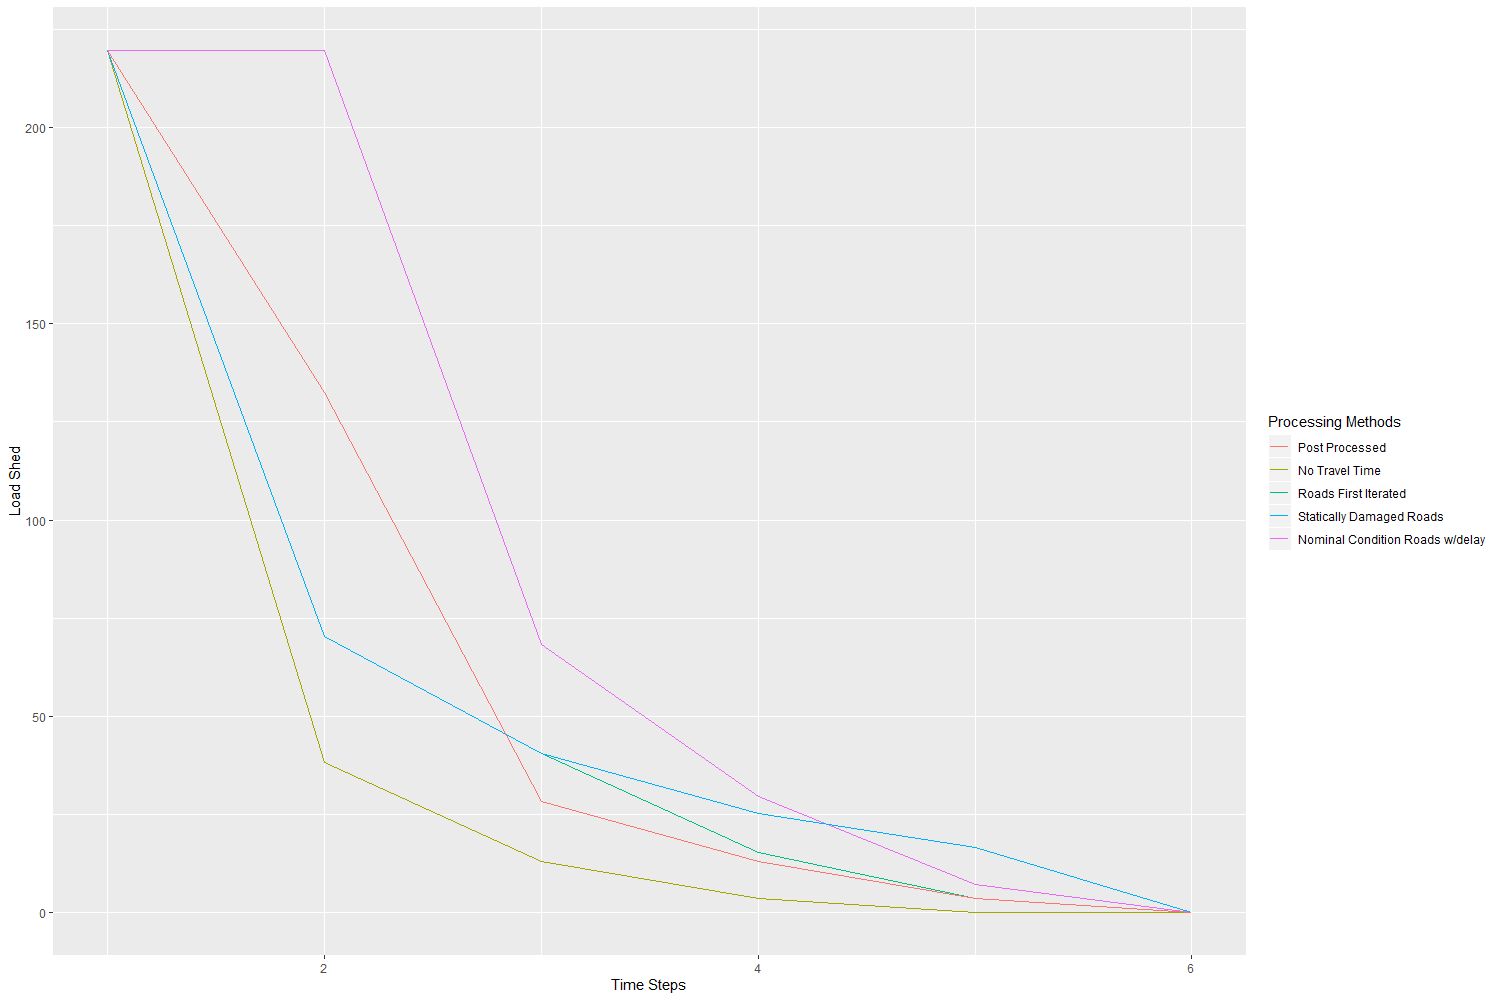
\includegraphics[width=.9\linewidth]{Rplot30Rand.png}9
		\caption{Load Shed by shift in the 30 bus randomized damage scenario}
		\label{fig:sub1}
	\end{figure}

	We can draw comparable conclusions to the the geographically distributed base case, but for this scenario, the post-processing heuristic suggests a lower total load shed. This seems to be due to the first several node and edge repairs being overwhelmingly obvious choices, but even given the rapid drop to baseline, the total lost load over the repair horizon is $406.8$ MW-shifts as compared to the $349.2$ of solving the roads first or the $274.4$ of the lower bound solution.
	
	To demonstrate that the changes to how the road grid is treated drive much of the changes in satisfied power flow, we display the schedule for the case below for each of it's solution methods. Of note is that not every element is repaired due to redundancies, but that is fine in the context of disaster response as the first priority is satisfying demand and restoring redundant systems is a lower priority. 
	
	 \begin{table}[htbp]
		\centering
		\resizebox{\columnwidth}{!}{\begin{tabular}{|c|c|c|c|}
			\cline{1-4}
			Shift Number & Road First & Nominal Roads & Post Processed\\
			1 & Node 4, Line 2, Line 3 &Node 4, Line 2, Line 3, Line 17, Line 24 & Node 7, Line 17, Line 3 \\
			2 & Node 7, Line 8, Line 35 & Node 7, Node 23 & Node 4, Line 35 \\
			3 & Node 23, Node 24, Line 30 & Node 18, Node 24 &  Node 23, Node 24 \\
			4 &Node 18, Line 14, Line 17, Line 24 & Node 20, Line 30, Line 35, Line 8, Line 14 & Node 18, Line 30, Line 2, Line 8, Line 20\\
			5 & Node 15, Line 20 & & Node 15, Line 24, Line 14\\
			6 & & &  \\
			\hline
		\end{tabular}}
		\caption{Repair Schedule by interaction method}
		\label{time}
	\end{table}
	\subsubsection{Varied Roads}
	We now perturb the road topology of the network case and solve a slight variation of the base case on the new topology. The base-case road network was constructed with a Watts-Strogatz graph with neighbor connectivity 3 and global connectivity .03 as discussed earlier. To show the model as written is valid for all topologies, we permute the road network while keeping the power grid static. The replacement topology is another Watts-Strogatz graph with neighbor connectivity 2 and global connectivity .015 and distances between nodes increased by 25\%. This simulates the effect of the power grid in a more rural area or more distributed population clusters in a hurricane effected area.
	
	The solutions are as follows for first the unperturbed road network and then the perturbed road network.
	
	\begin{figure}[H]
		\centering
		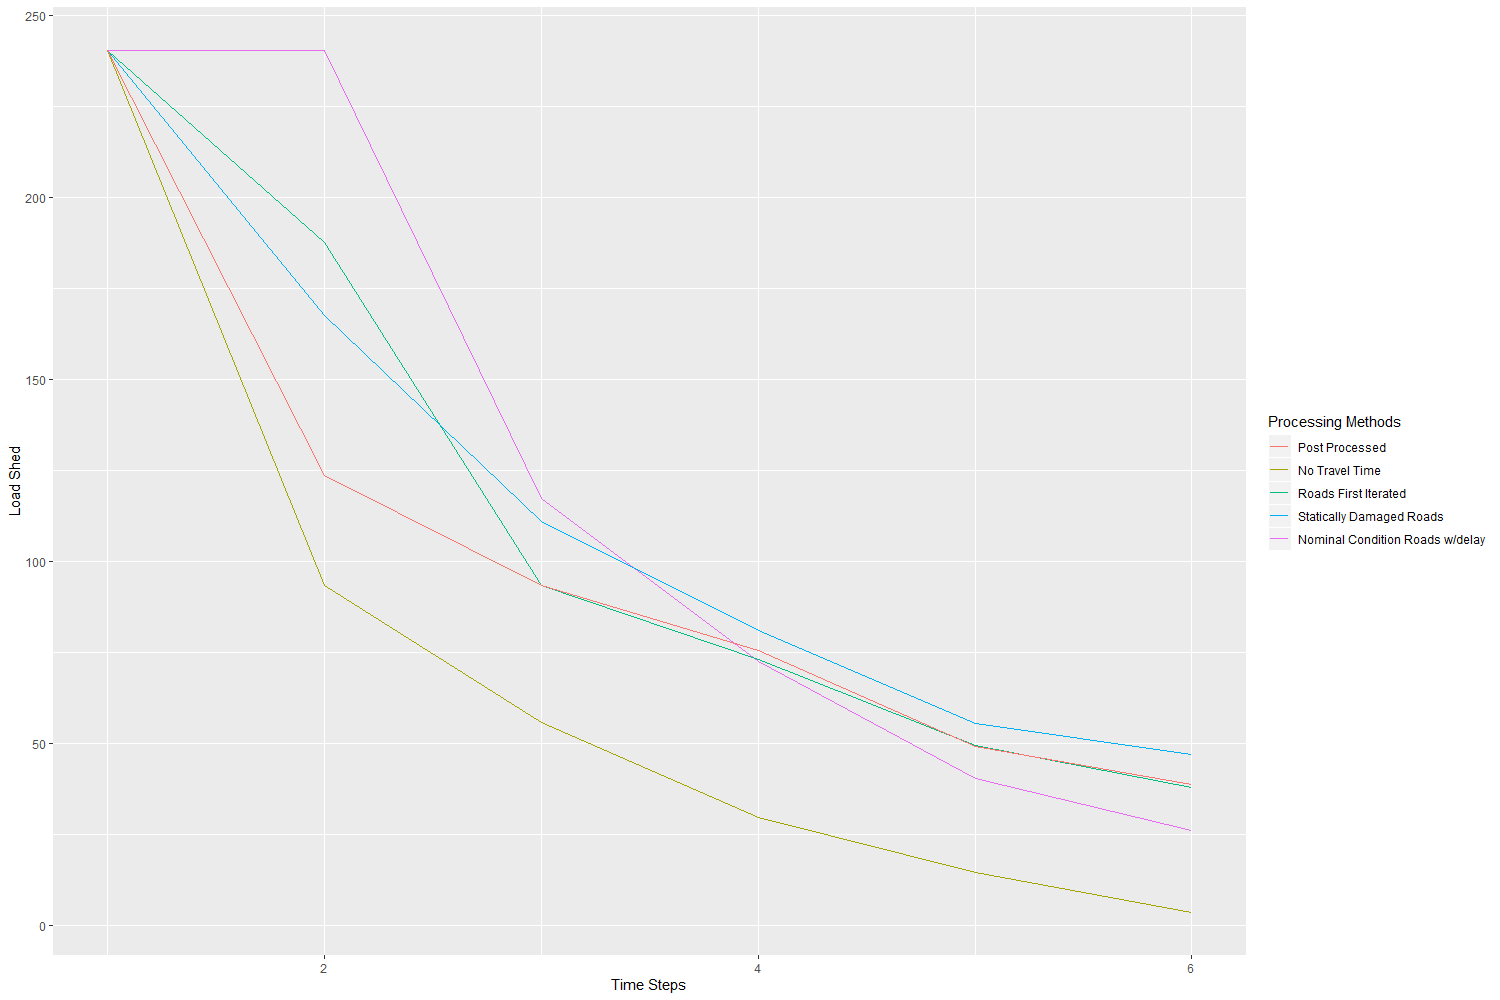
\includegraphics[width=.9\linewidth]{Rplot30Unperturbed.png}
		\caption{Load Shed by shift and method in the 30 bus scenario before road perturbation}
		\label{fig:sub2}
		
		
	\end{figure}
	\begin{figure}[H]
	\centering
	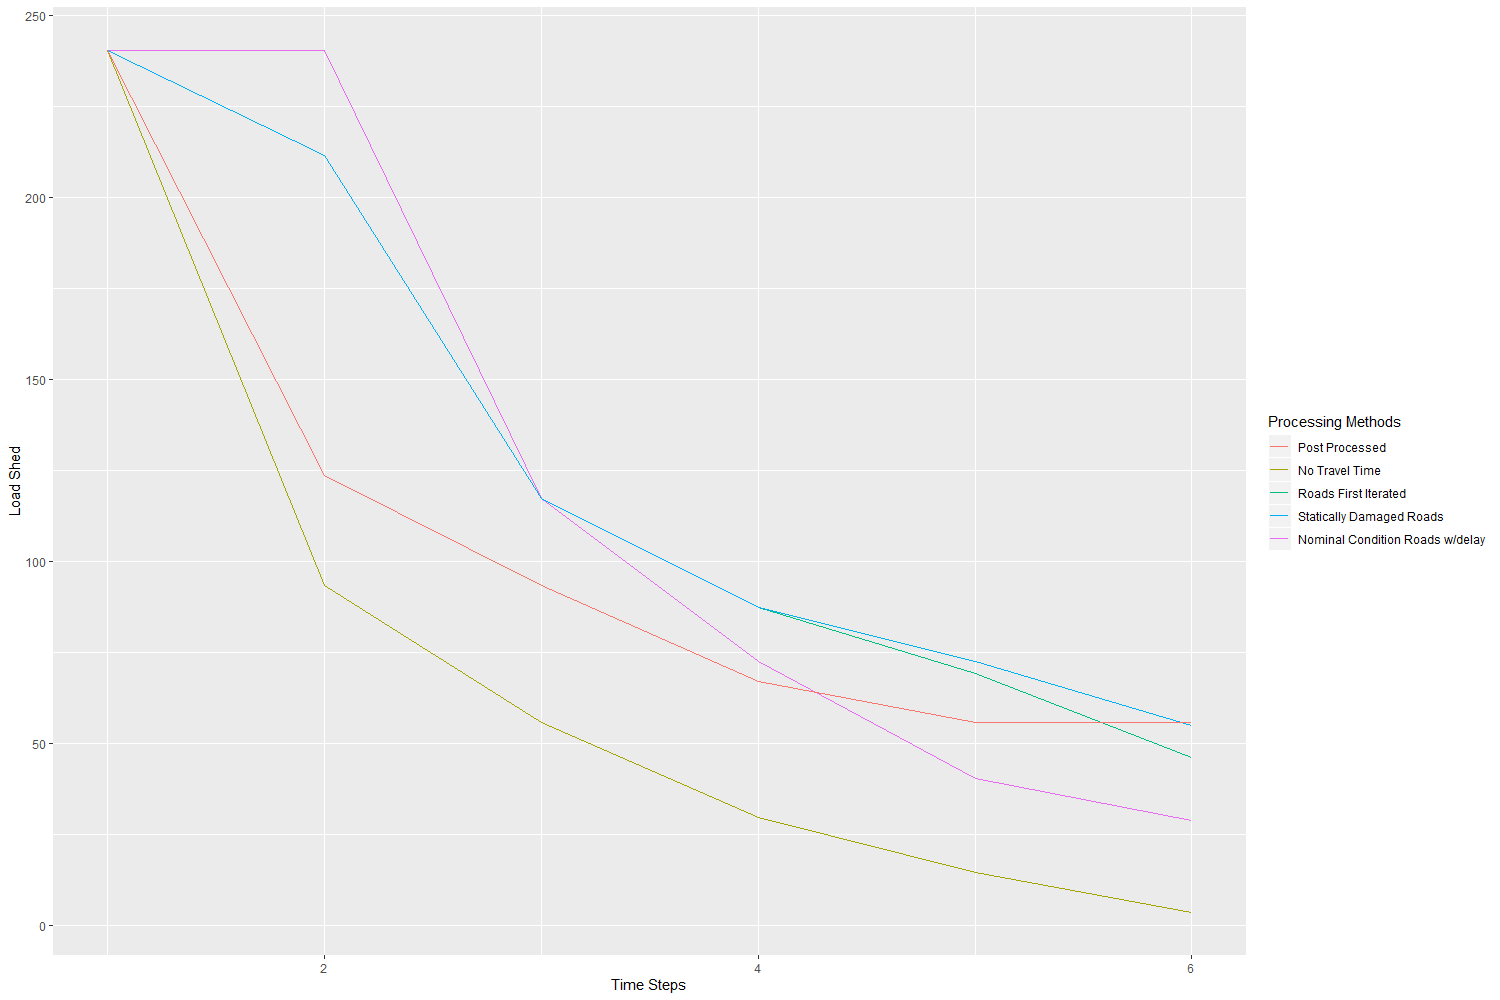
\includegraphics[width=.9\linewidth]{Rplot30Perturbed.png}
	\caption{Load Shed by shift and method in the 30 bus scenario after road perturbation}
	\label{fig:sub2}
	
	
	\end{figure}
	
		We get largely intuitive changes here. Interaction frameworks that are on-face more sensitive to road changes have larger magnitudes of change in performance under perturbation of the road network. When the road network is expanded, the framework where road repair is ignored and the roads are treated as statically damaged performs worse by comparison to other frameworks.
	
	Of note here is that the heuristically solved version of the model without travel time and use of a post-processor performs much better (i.e closer to the lower bound) in the case with the road network perturbed to be more distant. This is likely to be because the heuristic ignores road repair entirely in the name of not having to solve a mixed integer programming model. A version of the model where the road repair integer program is solved and used to generate time dependent road lengths would likely be significantly closer
	
	\subsubsection{Varied Damage Intensity}
	We now perturb the base case for both lower and higher damage scenarios in order to show model effectiveness for varying levels of damage.
	\begin{figure}[H]
		\centering
		\includegraphics[width=.9\linewidth]{Rplot30scenario2.png}
		\caption{Load Shed by shift in the 30 bus scenario with increased damage}
		\label{fig:sub2}
		
		
	\end{figure}

	For larger amounts of damage on a network, the repair curve has a large initial drop followed by the same amount of tailing off seen in lower damage cases. This is likely because of most power grids having a few high priority 
	\subsubsection{Varied Grid Topology}
	We now perturb the base case to a larger and more complex power grid in order to confirm model validity 
	\begin{figure}[H]
		\centering
		\includegraphics[width=.9\linewidth]{Rplot57.png}
		\caption{Load Shed by shift in the 57 bus scenario}
		\label{fig:sub2}
		
		
	\end{figure}
	
	While the result for both solving the roads first and for solving with nominal condition roads with delay have similar performance to previous cases demonstrating model interactions, the heuristic solution method of solve and post-process performs significantly worse. The reason for this is likely that a geospacially larger power grid means that routing is a proportionally larger share of each shift, and ignoring that component until postprocessing results in worse solutions the spatially larger the grid gets.
	
	\subsection{Overall}
	From the basket of demonstrated scenarios, we can see that interaction frameworks that allow more information sharing between road and power repairs are closer to the theoretical lower bound (i.e better solutions for the power grid) are better across the board. As we make the assumption that power repairs that get to operate on a road network that has been repaired to their needs requires a one shift delay in the start of repair operations, it's subpar compared to solving the road network and then interleaving the power repairs in with that. Were that assumption not to be valid, solving the power grid repairs under the presumption of nominal condition roads and then using those solutions to find a series of road repairs would be the best way of solving it. There are real reasons to give the road grid first-mover priority (e.g prioritizing flow in of humanitarian goods rather than restoration of power grid operations), but even under that interaction framework, power grid outcomes are better than they were under the schedule and post-process framework.
	\section{Resilience}
	\subsection{Introduction}
	Given that we've constructed a model for response to a scenario of a hurricane strike on a grid, we can use this to look at how different methods of resilience. By generating test cases and then making the grid resilient through either traditional hardening or by forming microgrids as has become popular in electrical engineering literature. 
	
	Most approaches to resilience construct a resilience curve like the following from \cite{Madni2020} (Image licensed to creative commons):
	
	\begin{figure}[htbp]
	\centering
	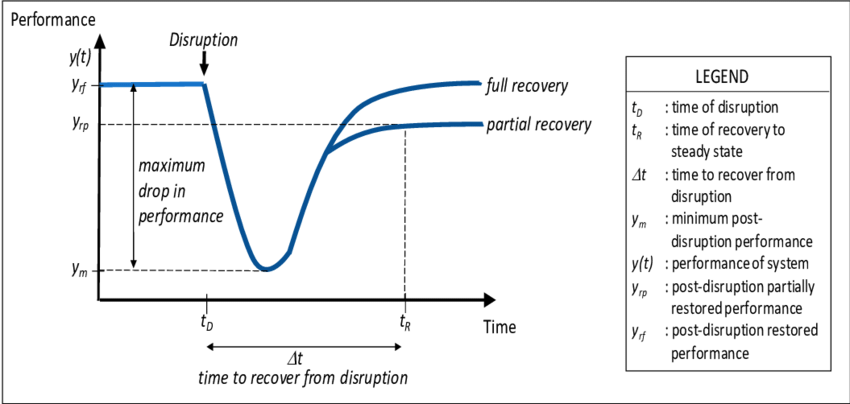
\includegraphics[width=.9\linewidth]{resiliencecurve.png}
	\caption{Standard depiction of resilience curves}
	\end{figure}
	
	Most literature assumes the recovery phase for a system is fixed so they study resilience in the context of minimizing either time to restoration of system performance or minimizing the severity of the initial drop. As we've been working with models for repair of damaged networks the generation of repair curves showing both lost road over time as well as power demand shed over time can be transformed into a steady state plus recovery curve as depicted above. This method gives us both the magnitude of the drop and the time to recovery as well as the curve that it generates. Using this, we elect to look into how the earlier defined repair model interacts with standard methods of improving resilience of a power grid.
	
	\subsection{Hardening}
	
	Hardening is one of the approaches to resilience by fortifying a subset of nodes and edges in a network to make it harder to damage. In the context of a power grid, this can be anything from sticking additional support guide wires on power poles to burying lines to building flood walls and windbreaks around substations. Traditionally this is looked at in the context of interdiction problems \cite{ChurchEA2007}. To overview the problem solved in hardening: player 1 operates a network, player 2 attacks the network with the objective of minimizing maximum flow, player 1 hardens the network before the attack under the assumption that it's coming and wants to preserve as much of the network's capacity as possible. This is typically formulated as a trilayer max/min/max mixed integer programming \cite{Mahmoo2016}, but it can be approached as a stochastic problem with uncertainties used to model attacks not being guaranteed to succeed \cite{Ramirez2009}.
	
	A similar approach can be taken with disaster planning. Unlike in multi-actor interdiction, the attack coming from a hurricane is a random process of nature and not a targeted interdiction by an intelligent actor. When solving this problem, finding a fixed quantity of damage equal to the ability to fortify under budget constraints that minimizes maximum flow allows for planning of network hardening. Solving this to optimality with best practices requires a delve into bi-level optimization that is outside the scope of this thesis. We therefor solve the problem heuristically through the following setup.
	
	\begin{enumerate}
		
	\item Solve baseline DC-OPF for the given power grid
	\item identify how many nodes (n) and edges (e) to be fortified
	\item select at least the 2n highest demand nodes and the 2e highest utilization edges
	\item for each subset of nodes/edges of the correct size, solve DC-OPF with those elements damaged
	\item find the minimum demand satisfied and use those damaged elements as the fortified elements when analyzing resilience 
	\end{enumerate}

	This is heuristically solved rather than guaranteed to be solved to optimality, but in the limit where all possible subsets are considered, this is a full solution of the multilayer optimization problem by enumeration that finds the set of attacked elements that minimizes maximal power flower. 
	\subsection{Results}
	We elect to use the 30 bus network and bus 57 networks outlined earlier to demonstrate the effectiveness of targeted fortification vs untargeted resilience. We construct a basket of scenarios randomly where each scenario reflects 50\% line loss and 25\% bus loss in the power grid and a standardized road damage of 50\%. Each scenario is then solved thrice. Once with a set of resilient elements as chosen above with the interdiction problem solved, once with fortification chosen based on highest power demand buses and highest use edges as defined by the ratio of flow in the undamaged case to maximum allowable flow as a plausible approximation that a power utility would use, and then again without any hardening to provide a base case for comparison.
	
	Solution here is done to optimality for the interdiction as these networks are small and therefore computational time is small (90 minutes on a desktop with i7 processor) to solve to optimality, but the heuristic methods outlined above are valid for analysis of larger networks, though the literature base will have more sophisticated heuristics and metaheuristics to approach interdiction.
	
	For the interdiction driven case, nodes 7 and 1 are hardened as are edges (22,23), (5,9), (1,5), and (0,1). For the version where the highest load buses and edges are chosen, nodes 4 and 7 are hardened as are edges (22,23), (5,9),(23,24), and (14,17).
	
	From this we then run 10 randomized scenarios as outlined above to properly display the difference in not just recovery time, but amount of unsatisfied demand during the repair process for different treatments of resilience.
\begin{figure}[htbp]
	\centering
	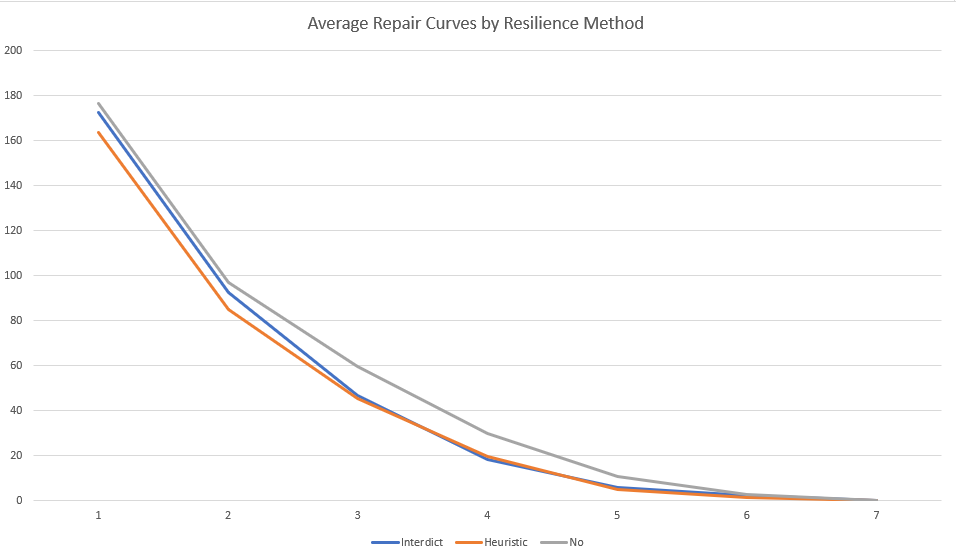
\includegraphics[width=.9\linewidth]{AverageSpaghetti.png}
	\caption{Average load loss over a set of random scenarios by resilience method}
\end{figure}
	
\begin{figure}[htbp]
	\centering
	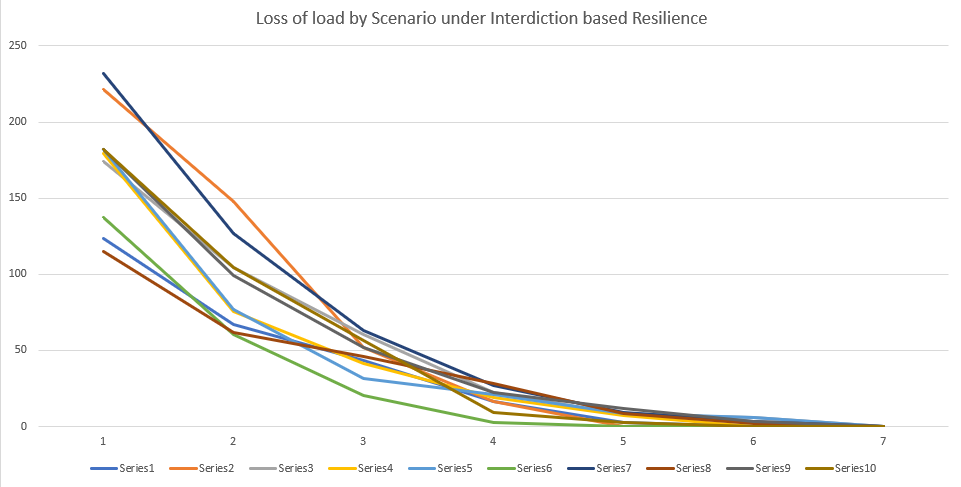
\includegraphics[width=.9\linewidth]{OptimalResilienceSpaghetti.png}
	\caption{Repair load loss curves by scenario under interdiction-based resilience planning}
\end{figure}
	\begin{figure}[htbp]
		\centering
		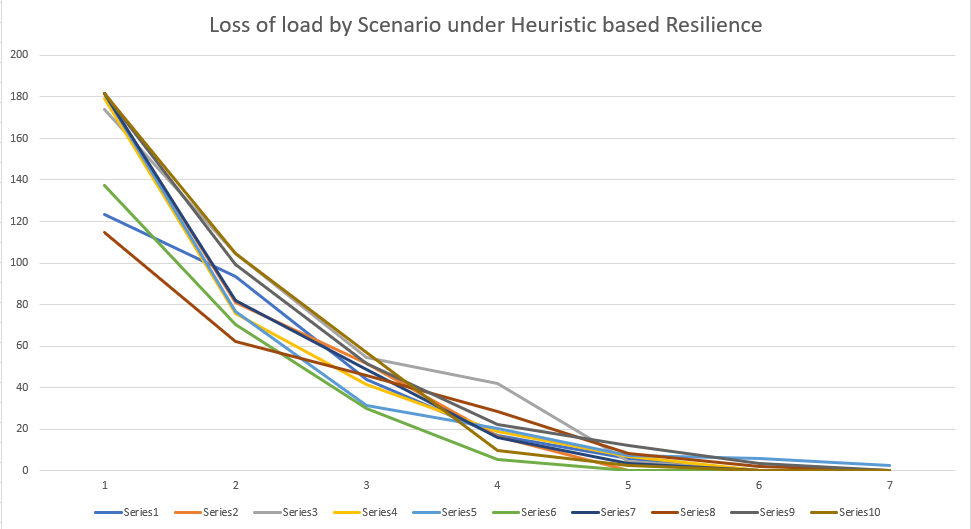
\includegraphics[width=.9\linewidth]{HeuristicResilienceSpaghetti.png}
		\caption{Repair load loss curves by scenario under heuristic-based resilience planning}
	\end{figure}
\begin{figure}[htbp]
	\centering
	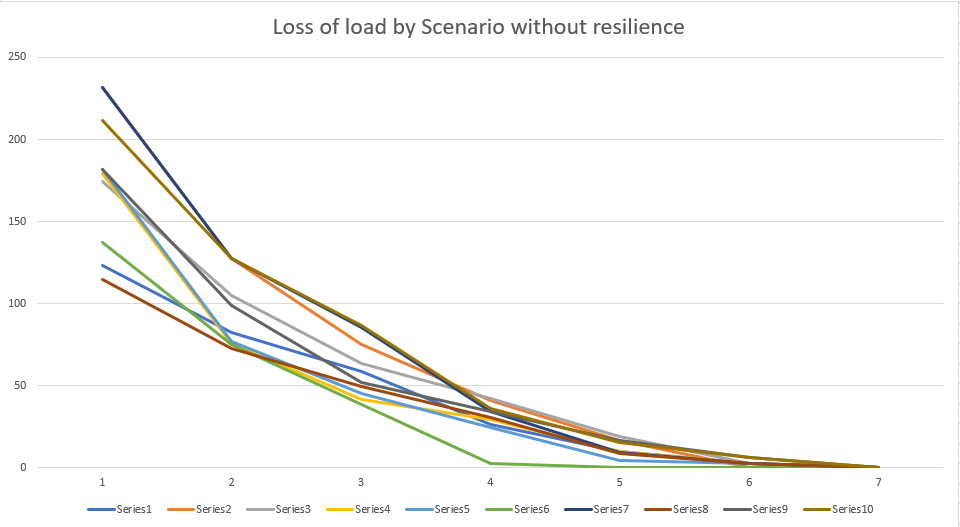
\includegraphics[width=.9\linewidth]{NoResilienceSpaghetti.png}
	\caption{Repair load loss curves by scenario under no resilience planning}
\end{figure}
	 \begin{table}[htbp]
	\centering
	\resizebox{.75\columnwidth}{!}{\begin{tabular}{|c|c|c|c|}
			\cline{1-4}
			Shift Number & Interdiction Based & Heuristic Based & No Resilience\\
			1 & 172.8 & 163.8 & 176.8\\
			2 & 85.9 & 91.7 & 96.9\\
			3 & 46.7 & 45.6 & 59.5\\
			4 & 18.5 & 19.6 & 30 \\
			5 & 5.8 & 5.12 & 10.8\\
			6 & 2.11 & 1.17 & 2.6\\
			7 & 0 & 0.24 & 0\\
			total & 331.7 & 327.13 & 376.5\\
			\hline
	\end{tabular}}
	\caption{Average unsatisfied demand by shift by resilience methods}
	\label{time}
\end{table}


	When using this interacted road model to look at resilience in the context of the shape of the repair curve and not just initial drop or time to return to normalcy, we find that over the average of the set of random scenarios modeled interdiction based resilience has lower total load shed, but using the ratio heuristic for selecting power lines and the load heuristic for selecting edges results in a resilience strategy that has a smaller magnitude of initial drop in power demand satisfied. Both of them are substantially better than doing nothing as would be intuitively expected, but the difference between use of a heuristic and solution to the full interdiction problem is much less intuitive in so far as a heuristic yeilds better results than the interdiction based method that is lauded in literature for hardening of grids. In suspicion of this being an anomalous result due to the budget constraint or grid topology based on choices of what elements to fortify, we repeat the process under a different budget constraint. We elect this time to fortify only one node and three edges choosing node 1 and edges (1,5), (22,23), and (0,1) for the interdiction based fortification and node 4 with edges (22,23), (22,24), and (5,9) for the heuristic based fortification. We repeat the simulation of random damage with the same parameters for random damage as before.
	
	Skipping visualization of the suite of repair curves as they look very similar to the ones above in figures 10-12, we show the average resilience curve for each of the 3 resilience methods below.
	
\begin{figure}[htbp]
	\centering
	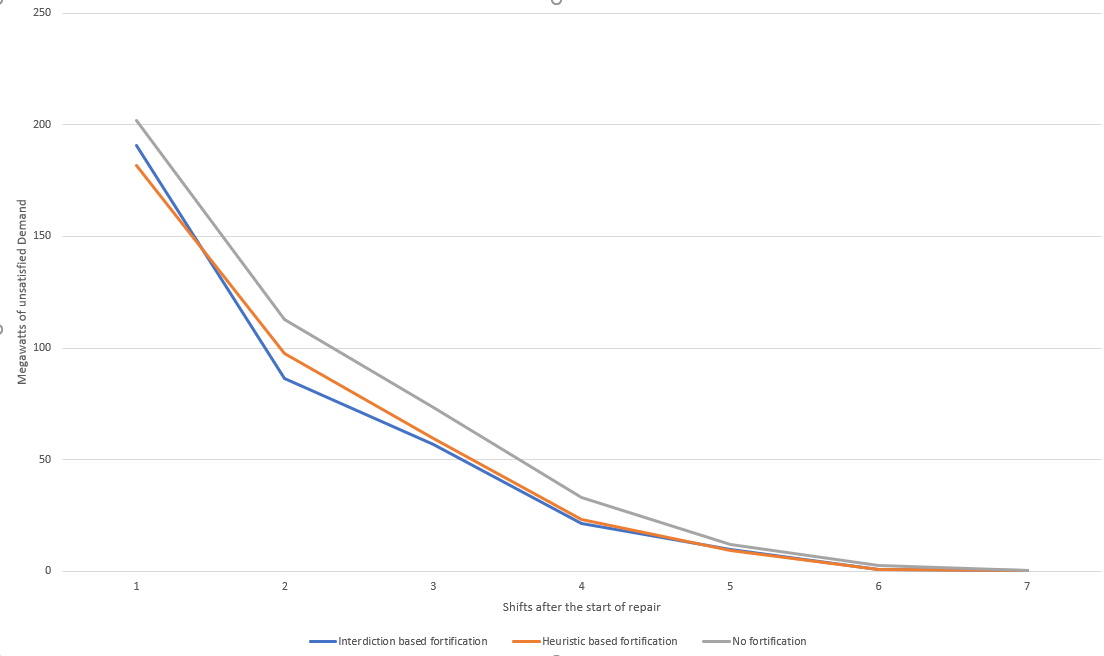
\includegraphics[width=.9\linewidth]{LowBudgetSpaghetti.png}
	\caption{Average repair curve for the tightened budget constraint}
\end{figure}
	 \begin{table}[htbp]
	\centering
	\resizebox{.75\columnwidth}{!}{\begin{tabular}{|c|c|c|c|}
			\cline{1-4}
			Shift Number & Interdiction Based & Heuristic Based & No Resilience\\
			1 & 190.6 & 181.8 & 201.8\\
			2 & 86.2 & 97.5 & 112.9\\
			3 & 56.8 & 59.6 & 73.3\\
			4 & 21.5 & 23.1 & 33 \\
			5 & 9.56 & 9.19 & 12.0\\
			6 & 0.94 & 0.92 & 2.46\\
			7 & 0.22 & 0.22 & 0.22\\
			total & 365.8 & 372.2 & 435.7\\
			\hline
	\end{tabular}}
	\caption{Average unsatisfied demand by shift by resilience methods}
	\label{time}
\end{table}

Once again, we see the same pattern of heuristically chosen and interdiction chosen fortification being similar with heuristic fortification having a smaller initial drop and the interdiction based fortification having a slightly smaller total load shed.  

The takeaway from these two example studies into resilience is that the shape of the repair curve does matter for resilient operations and is responsible for the difference in outcomes for the two methods of choosing fortified elements on a the topology. As we see from comparing the interdiction based resilience to the heuristically driven resilience method, initial drop and time to full operations aren't the only things that matter. As interdiction based resilience is most frequently used in defense of a network against a directed attack and not a random event like a hurricane, it may not be the best tool for the job in planning resilience against a random event. We suspect this to be a place where probability based resilience (harden/fortify the elements most likely to be damaged based on assessment of hurricane forecasts) or some form of two step stochastic optimization to construct a resilience plan. 

	\section{Conclusions}
	
	As discussed back in the literature review, interaction between actors in a repair context is not well explored in the literature. We present a pair of models and analyze several perturbations of standard IEEE test grids to demonstrate the effectiveness of interacting the models in several different frameworks. This yields a series of results that are closer to a theoretical lower bound as compared to treating repairs as a pure scheduling problem on the power grid and applying routing as an after-the-fact post processing step as is done in previous modeling efforts that generate only a schedule and leave routing to the agency conducting repairs.
	
	These repair models are then extended into resilience models to show that interdiction based modeling performs better than a heuristic method at minimizing the unsatisfied power demand over a basket of random damage instances. This suggests that further consideration of multiple network layers can lead to better insights when considering resilience planning of multiple network layers.
	

	\subsection{Future Research Directions}
	The clear low hanging fruit for future research directions is to take the models outlined and fit them to the topology of a real place and then simulate a hurricane strike to generate the damage scenario. This would require an involved effort to correctly model both flooding/storm surge as well as wind damage, but is possible. Additionally along the same line of research, treating the repair problem outlined above as a recourse step in a two stage stochastic program based on a suite of scenarios. The first step could take the form of inventory location and quantity or alternatively a problem about network hardening.
	
	Another research direction that could be undertaken is to account for imperfect information about the state of the power grid or imperfect information about the status of the road network. Sharing of resources (e.g space on a truck moving supplies in) as a form of optimization under uncertainty which would also have implications for more interesting interactions between actors in the repair effort. Along those lines, optimization of roads has implications for other types of network infrastructure such as water supplies and rail/mass transit networks.
	\section{Bibliography}
	\bibliographystyle{apalike}
	\bibliography{sources}
\end{document}